
\documentclass[../main.tex]{subfiles}
\begin{document}
\section{Results}
The CHIPS project used the Fujitsu 55nm process to fabricated the final chip. Each chiplet used the Synopsys design compiler to synthesize its design. Then, the chiplet used the Cadences Innovus tool to place and route the design. VCS was used to verify the functionality of the post place and routed chiplets. Cadences Tempest timing tool was used to verify the hold and setup timing in the post place and routed design. Cadence Voltus tool was used to get dynamic and static power of each chiplet. Ones each chiplet was placed and routed, the top-level design, including each chiplet and IO driver, was pushed through the same process. Figure 1 shows the final CHIPS layout. The final chip core clock frequency is around 50MHz and has a size of 10mm by 10mm and an area of 100mm\textsuperscript{2}. Table 1 shows the size, area, and power for each of the chiplets.

\begin{figure}
    \centering
    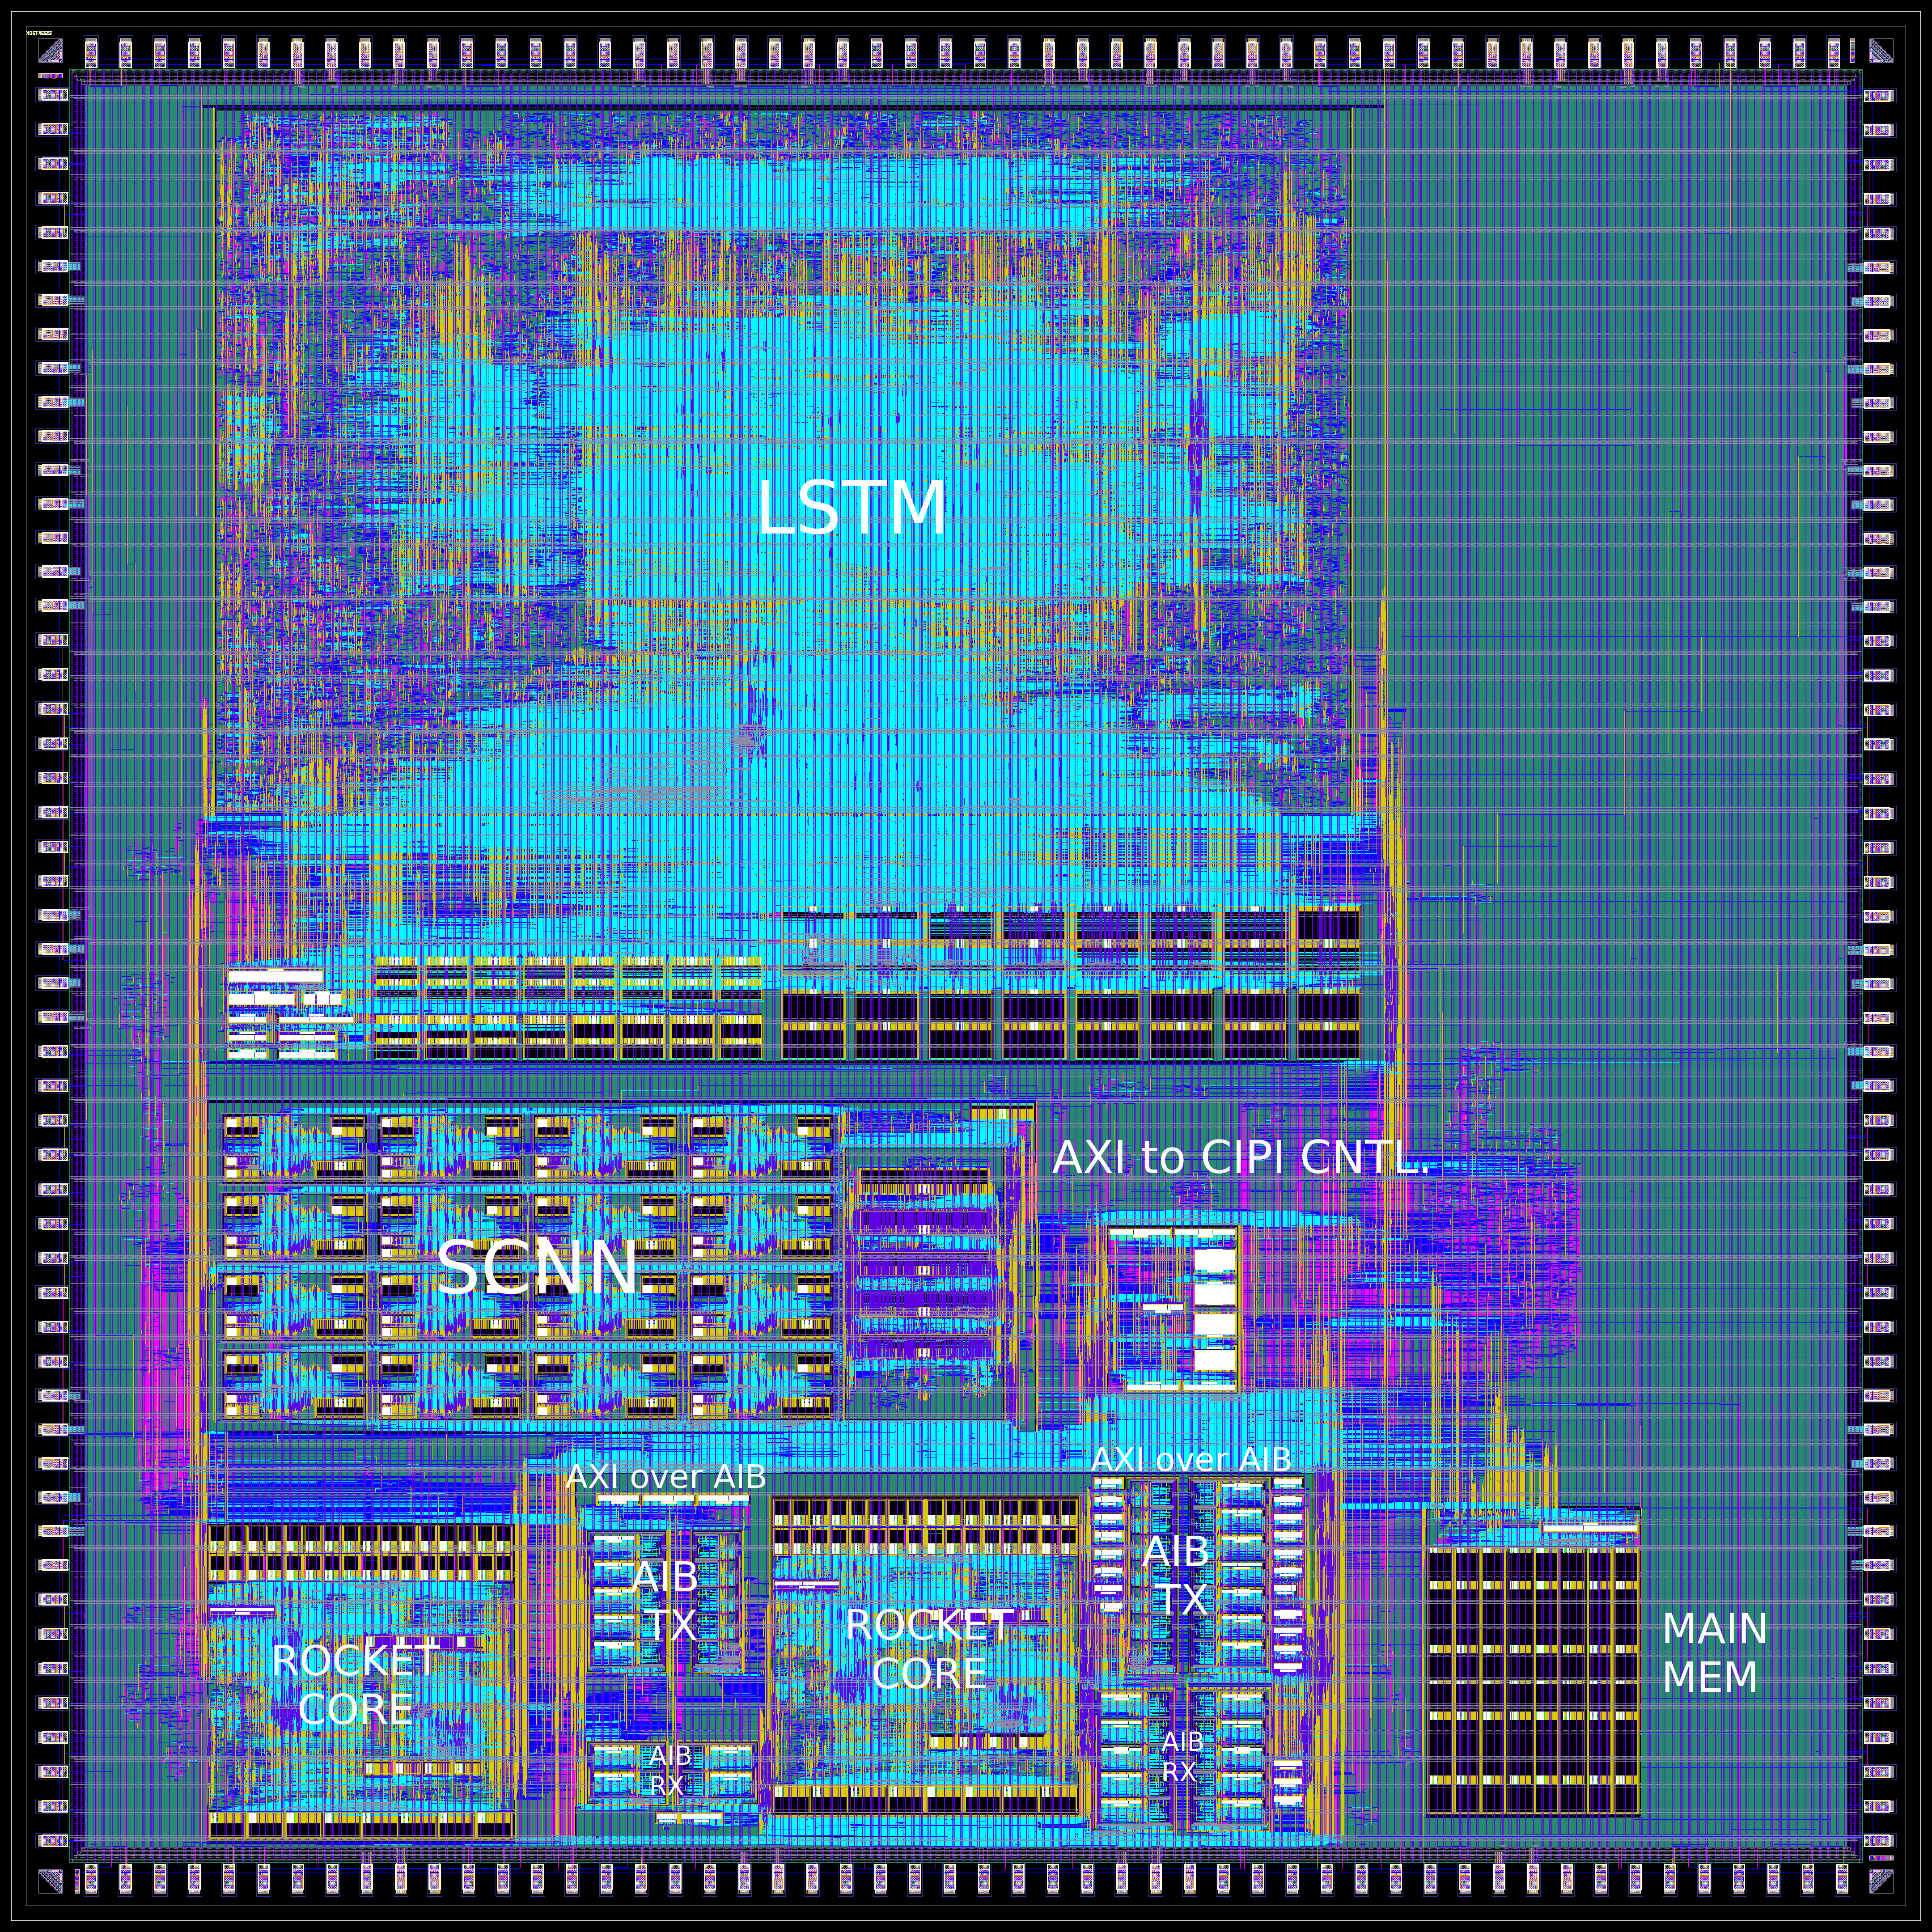
\includegraphics[scale=.06]{pngs/CHIPS-Layout.png}
    \caption{CHIPS Layout}
    \label{fig:CHIPS-layout}
\end{figure}

\end{document}